% !TeX TS-program = xelatex

\documentclass{beamer}
%Set the slide theme
%Change to meet your taste
% Madrid, Copenhagen, Berlin, ... works
\usetheme{metropolis}


\usepackage{xecolor}
\usepackage{amsmath}
%\usefonttheme[onlymath]{serif} %Change the math font

\usepackage{xepersian}
\settextfont[Path=fonts/]{Parastoo}

%---------------------------------------------------------------------------------
% Seetings to force Beamer works with Xepersian and RTL typesetting
%-------------------------------------------------------------------------------
%\raggedleft

% For right to left lists (itemize and enumerate)
\makeatletter
\newcommand{\RTList}{\raggedleft\rightskip\@totalleftmargin}
\makeatother
% Correct the bullet for RTL texts
\setbeamertemplate{itemize item}{\scriptsize\raise1.25pt%
 \hbox{\donotcoloroutermaths$\blacktriangleleft$}} 

% To force beamer use numbering in captions
\setbeamertemplate{caption}[numbered]{}% Number float-like environments



%---------------------------------------------------------------------------------
\title{
	عنوان پروژه
}
\subtitle{}
\author{پرهام الوانی}
\institute{دانشکده مهندسی کامپیوتر و فناوری اطلاعات}
\date{پاییز ۱۳۹۶}

\begin{document}
\begin{persian}
%------------------------------------------
% Title page
%------------------------------------------
\begin{frame}
\maketitle
\end{frame}

% To adjust the paragraphs in RTL
\everypar{\rightskip\rightmargin}
%-------------------------------------------------------------------------------
\begin{frame}{طرح مساله}
	\begin{itemize}\RTList
		\item سمت کاربر
		\item سمت دیتاسنتر
		\begin{itemize}\RTList
			\item \lr{ETSI GS MANO}
		\end{itemize}
	\end{itemize}
\end{frame}
\begin{frame}{مساله اول}
	\par
	\lr{NFVO} وظیفه‌ی استقرار زنجیره‌های کارکرد سرویس را برعهده دارد.
	همانگونه که در مستند \lr{ETSI} نیز آمده است هر نمونه از کارکردهای مجازی شبکه نیاز دارد
	تحت مدیریت یکی از \lr{VNFM}های موجود در شبکه باشد.
\end{frame}
\begin{frame}
	\begin{center}\begin{figure}
		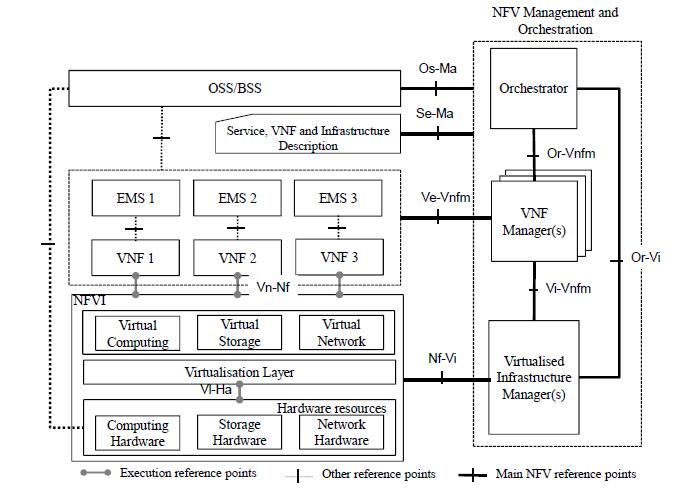
\includegraphics[scale=0.4]{images/nfv-arch.jpg}
		\caption{معماری سطح بالای مجازی‌سازی کارکردهای شبکه}
	\end{figure}\end{center}
\end{frame}
\begin{frame}
	\par
	یکی از وظایف \lr{VNFM} مانیتور کردن وضعیت و خطاهای نمونه‌ها می‌باشد
	این امر باعث افزایش بار پردازشی \lr{VNFM} می‌گردد
	و از سوی دیگر تحلیل این اطلاعات می‌بایست با تاخیر معقولی صورت پذیرد که این امر
	نیاز به یک بستر ارتباطی مطمئن دارد.
\end{frame}
\begin{frame}
	\par
	پذیرفتن بیشترین تقاضای زنجیره‌ کارکرد سرویس با در نظر گرفتن نیاز هر نمونه کارکرد مجازی شبکه به یک \lr{VNFM}.
\end{frame}
\begin{frame}
	\begin{itemize}\RTList
		\item توپولوژی زیرساخت شامل پنهای باند لینک‌ها و ظرفیت \lr{NFVI-PoP}ها موجود است.
		\item n تقاضای زنجیره‌ کارکرد سرویس به صورت کامل و از پیش مشخص شده داریم.
		\item هر تقاضا شامل نوع و تعداد نمونه‌های مجازی و پنهای باند لینک‌های مجازی می‌باشد.
		\item F نوع کارکرد مجازی شبکه تعریف شده است که هر یک مقدار مشخصی از حافظه را مصرف می‌کنند.
		\item تعداد پردازنده‌هایی که به هر نمونه تخصیص می‌یابد با توجه به ترافیک ورودی نمونه مشخص می‌شود.
		\item نمونه‌ها بین زنجیره‌ها به اشتراک گذاشته نمی‌شوند.
	\end{itemize}
\end{frame}
\begin{frame}
	\begin{itemize}\RTList
		\item محدودیت ظرفیت لینک‌ها
		\item محدودیت توان پردازش سرورهای فیزیکی با توجه به میزان حافظه و تعداد پردازنده‌ها
	\end{itemize}
\end{frame}
\begin{frame}
	\begin{itemize}\RTList
		\item برای سادگی مساله برای هر زنجیره یک \lr{VNFM} تخصیص می‌دهیم.
		\item \lr{VNFM}ها می‌توانند بین زنجیره به اشتراک گذاشته شوند.
		\item هر نمونه از \lr{VNFM}ها می‌تواند تعداد مشخصی از نمونه‌های کارکرد مجازی شبکه را سرویس دهد. 
		\item برای ارتباط میان هر نمونه از \lr{VNFM}ها و \lr{VNF}ها پهنای باند مشخصی رزرو می‌گردد.
		\item بر روی هر \lr{NFVI-PoP} حداکثر یک نمونه \lr{VNFM} مستقر می‌گردد.
	\end{itemize}
\end{frame}
\begin{frame}
	\begin{latin}\begin{thebibliography}{9}
		\bibitem{P11}
		Mohammad Abu-Ledbeh, Diala Naboulsi, Roch Glitho, Constant Wette Tchouati.
		\textit{On the Placement of VNF Managers in Large-Scale and Distributed NFV Systems}. 
		IEEE Transactions on Network and Service Management, 2017
	\end{thebibliography}\end{latin}
	\par
	هدف کاهش هزینه‌ی عملیاتی در حالی که تاخیرهای ارتباطی و محدودیت‌های ظرفیت رعایت می‌شوند.
\end{frame}
\begin{frame}{مساله‌ی دوم}
	\par
	مساله از منظر \lr{VNFM} برای \lr{scale} کردن یک \lr{VNF instance}
	زمانی که سیستم به صورت کامل مستقر شده است استفاده می‌گردد.
	این \lr{scale} کردن به دلیل تغییرات ترافیکی در سیستم به وقوع پیوسته است.
\end{frame}
\begin{frame}
	\par
	کمترین هزینه برای اعمال تغییرات بر روی دیتاسنتر.
	در اینجا منظور از هزینه، توان مصرفی سرورها و هزینه‌هایی است که جهت مهاجرت و ساخت نمونه‌ها پرداخت می‌شود.
\end{frame}
\begin{frame}
	\begin{itemize}\RTList
		\item توپولوژی زیرساخت شامل پنهای باند لینک‌ها و ظرفیت \lr{NFVI-PoP}ها موجود است.
		\item وضعیت \lr{NFVI-PoP}ها و نمونه‌هایی که روی آن‌ها مستقر است موجود است.
		\item وضعیت لینک‌های فیزیکی و لینک‌های مجازی که روی آن‌ها قرار دارند موجود است.
		\item تعداد نمونه‌های لازم از پیش مشخص است.
		\item با ایجاد نمونه‌های جدید ترافیک ورودی و خروجی نمونه‌ی اولیه بین نمونه‌های جدید تقسیم می‌گردد.
		\item تنها در مورد یک نمونه از یک زجیره بحث می‌گردد.
	\end{itemize}
\end{frame}
\begin{frame}
	\begin{itemize}\RTList
		\item نمونه‌ها به صورت عمودی مقیاس‌پذیر نیستند.
		\item محدودیت توان پردازشی سرورهای فیزیکی با توجه به تعداد پردازنده‌ها
		\begin{itemize}\RTList
			\item هزینه‌ی ساخت نمونه
			\item هزینه‌ی مهاجرت نمونه
			\item هزینه‌ی روشن کردن سرور جدید
		\end{itemize}
	\end{itemize}
\end{frame}
\begin{frame}
	\begin{latin}\begin{thebibliography}{9}
		\bibitem{P21}
		Vincenzo Eramo, Emanuele Miucci, Mostafa Ammar.
		\textit{An Approach for Service Function Chain Routing and Virtual Function Network Intance Migration in Network Function Virtualization Architecture}. 
		IEEE Transactions on Networking, 2017
	\end{thebibliography}\end{latin}
	\par
	کاهش توان مصرفی در یک ترافیک \lr{cycle-stationary}
	با مهاجرت و مقیاس‌دهی عمودی نمونه‌ها در وضعیت‌های ترافیکی مختلف
\end{frame}

\end{persian}
\end{document}